\chapter{Level2 processor and I/O data}

\begin{figure}[t]
\centering
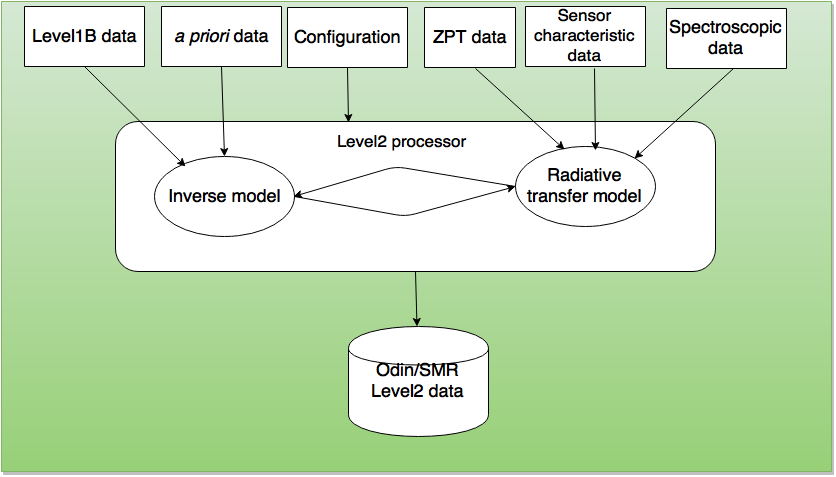
\includegraphics[width=14cm]{smr-level2-processor.png}
\caption{Schematic of the I/O data used and generated by the \smr\ Level2 processor.}
\label{fig:level2}
\end{figure}

\begin{figure}[t]
\centering
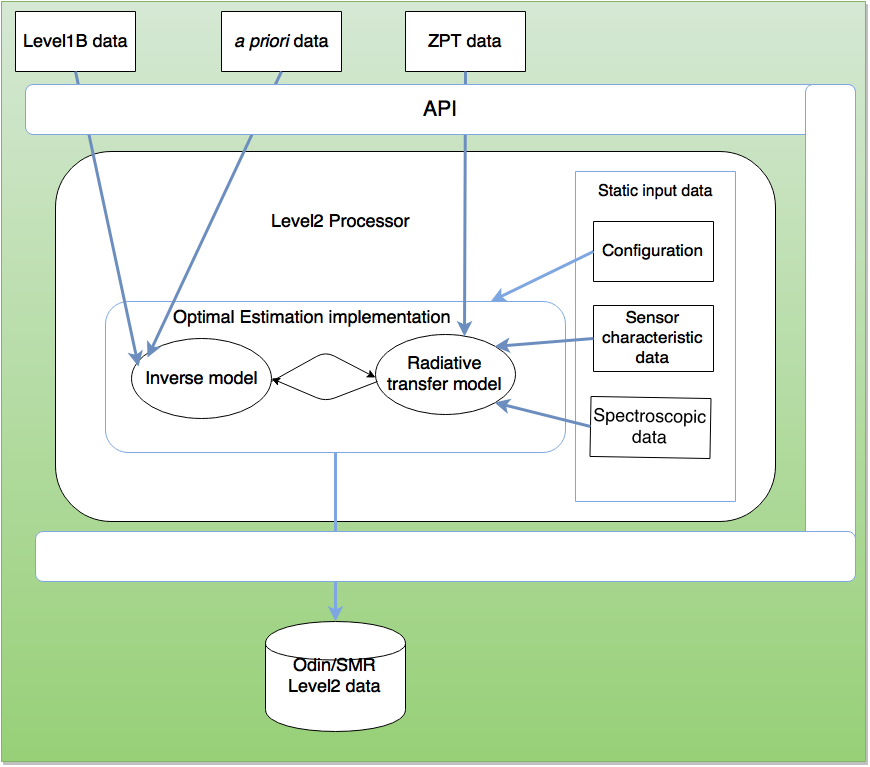
\includegraphics[width=14cm]{smr-level2-processor2.png}
\caption{Schematic of the I/O data used and generated by the \smr\ Level2 processor.}
\label{fig:level2b}
\end{figure}



\section{Level2 processor overview}

The \smr\ Level2 processor is designed to process
measurements from a scan of \smr\ in order to
retrieve profiles of atmospheric species.    
The Level2 processor is an optimal estimation method (OEM)
implementation, which combines measurement
information with Ancillary/Auxiliary data
and applies a forward model, and an iterative
scheme is used to find a best solution.   
The details of the algorithms within the
\smr\ Level2 processor is described in \smr\ Level2 ATBD.

\section{Level2 processor input data}

Figure~\ref{fig:level2} describes, on a high level, the input data used
by the Level2 processor and the generated output data.
The input data can be divided into two groups,
dynamic (or semi-dynamic) and static input data,

\begin{itemize}
  \item dynamic (or semi-dynamic) input data:
  \begin{itemize}

    \item \emph{Level1B data}: the most basic input data to the 
    Level2 processor is the Level1B data, i.e. geolocated and 
    calibrated spectra from a scan of \smr.
    
    \item \emph{Climatological \textit{apriori} data}:
    climatology data, covering all species of interest is required, as
    the OEM implementation needs a starting estimate for each profile
    to be retrieved. The climatology cover vertical, seasonal,
    and latitudinal variations of each species and is based on data
    from ?.

    \item \emph{ZPT data}:
    The Level2 processor requires external ZPT data (altitude, pressure, temperature)
    data. The ZPT data is extracted from the ERA-Interim dataset for the geolocation
    of the scan. ERA-Interim is a global atmospheric reanalysis from 1979, and
    data is available throughout the Odin mission.
  \end{itemize}
  \item static input data:
  \begin{itemize}
    \item \emph{Sensor characteristic data}:
    The forward model simulation of the Level2 processor takes into account
    sensor characteristic data, i.e. the antenna angular response,
    sideband filtering, and frequency response of each spectrometer channel.

    \item \emph{Spectroscopic data}:
    Spectroscopic data is basic input to the forward model of the Level2
    processor.

    \item \emph{Configuration}:
    \smr\ applies a number of different observation modes,
    and for each mode a different configuration is applied
    of the Level2 processor...
  \end{itemize}
\end{itemize}


The Level2 processor obtains the dynamic 
and semi-dynamic input data through a hierarcical
REST API, and the API is described in Sect.~\ref{sec:api}.
The static input data is integrated into the
Level2 processor, as described in Figure~\ref{fig:level2b}. 
%\smr\ applies a number of different observation modes,
%but the Level2 processor is identical for the various modes,
%in terms of the high level workflow.
The detailed data formats of the dynamic 
and static data are described in 
Sect.~\ref{sec:api} and Sect.~\ref{sec:static}.


\clearpage
\newpage
\subsection{API and dynamic input data}
\label{sec:api}

The Level2 processor obtains dynamic input data through
a hierarcical REST API, where deeper URIs return more
specific data.  All call URIs have a common root \url{rest_api/<version>}, which
has been omitted below for clarity.  All GET calls return JSON objects unless
otherwise noted. Key/value pairs are listed as name of the key
along with the type of the corresponding value within parantheses, followed
by a brief description of the contents.  
%See the sections on the different
%data sources for specifications on the structure of their respective JSON
%objects.

The URI hierachy is organized in the following way:
\begin{itemize}
    \item \url{freqmode/<date>/}: Returns object, which describes which frequency modes that were deployed the
    given date
    \begin{itemize}
        \url{freqmode/<date>/<backend>/<freqmode>/}: Returns object, which describes log data of the scans
        for the given date and deployed frequency mode
        \begin{itemize}
           \item \url{scan/<backend>/<freqmode>/<scanID>/}: Returns object that describes Level1B data for a given scan       
           \item \url{ptz/<date>/<backend>/<freqmode>/<scanID>/}: Returns object that describes ptz data for a given scan
           \item \url{apriori/<species>/<date>/<backend>/<freqmode>/<scanID>/}: Returns object that describes \textit{a priori} data for a given scan
        \end{itemize}  
    \end{itemize}
\end{itemize}
  

\subsubsection{Level1B overview data}
\subsection*{\url{freqmode/<date>/}}
Method: \emph{GET}

Returns object, which describes which frequency modes that were deployed the
given date (YYYY-MM-DD), with the following attributes:
\begin{itemize}
    \item Info:

        A list of objects containing information about which
        frequency modes that were mesured this date. 
        Each object contains the following keys:

        \begin{itemize}
            \item Backend \emph{(String)}: The backend for the data
            \item FreqMode \emph{(Int)}: The frequency mode for the data
            \item NumScan \emph{(Int)}: The number of available scans
            \item URL \emph{(URI)}: A URI 
                for getting more specific of the available scans\\ 
                 (\url{freqmode/<date>/<backend>/<freqmode>/})
        \end{itemize}
\end{itemize}

\subsection*{\url{freqmode/<date>/<backend>/<freqmode>/}}
Method: \emph{GET}

Returns object, which describes log data of the scans  
for the given date, backend, and freqmode,
with the following attributes:

\begin{itemize}
    \item Info:

        A list of objects that describes each scans
        with some log data.  
        Each object contains the following keys:

        \begin{itemize}
            \item AltEnd \emph{(float)}: Tangent point altitude ([\,m\,]) for last spectrum in scan
            \item AltStart \emph{(float)}:Tangent point altitude for first spectrum in scan
            \item DateTime \emph{(str)}: Mean UTC datetime (datetime(first) + datetime(last))/2 of scan
            \item FreqMode \emph{(Int)}: Deployed frequency mode
            \item LatEnd \emph{(float)}: Latitude of tangent point for last spectrum in scan
            \item LatStart \emph{(float)}: Latitude at tangent point for first spectrum in scan
            \item LonEnd \emph{(float)}: Longitude of tangent point for last spectrum in scan
            \item LonStart \emph{(float)}: Longitude at tangent point for first spectrum in scan
            \item MJDEnd \emph{(float)}: Modified julian date for last spectrum in scan
            \item MJDStart \emph{(float)}: Modified julian date for first spectrum in scan
            \item NumSpec \emph{(int)}: Number of atmospheric spectra in scan
            \item ScanID \emph{(int)}: Satellite time word identifier of scan
            \item SunZD \emph{(float)}: Mean solar zenith angle  (SunZD(first) + SunZD(last))/2 for scan
            \item URLS a list of key/value describing URIs containing
            more detailed data
            \begin{itemize} 
                \item URL-apriori-<species> \emph{(URI)}: 
                A URI for getting \textit{a priori} data of the scan\\
                (\url{apriori/<species>/<date>/<backend>/<freqmode>/<scanID>/})
                \item URL-ptz \emph{(URI)}: A URI for getting ptz data for the scan\\
                (\url{ptz/<date>/<backend>/<freqmode>/<scanID>/})
                \item URL-spectra \emph{(URI)}: A URI for getting Level1B spectra of the scan\\         
                (\url{scan/<backend>/<freqmode>/<scanID>/})        
            \end{itemize}
       \end{itemize}   
\end{itemize}

\subsubsection{Level1B data}
\subsection*{\url{scan/<backend>/<freqmode>/<scanID>/}}
Method: \emph{GET}

\subsubsection{PTZ data}
\subsection*{\url{ptz/<date>/<backend>/<freqmode>/<scanID>/}}
Method: \emph{GET}

Returns an object that describes the ptz data of the scan,
with the following attributes:

\begin{itemize}
    \item Pressure \emph{(array of doubles)}: Pressure vector ([\,Pa\,])
    \item Temperature \emph{(array of doubles)}: Temperature vector([\,K\,])
    \item Altitude \emph{(array of doubles)}:  Altitude vector([\,m\,])
    \item Latitude \emph{(double)}: Latitude of PTZ data
    \item Longitude \emph{(double)}: Longitude of PTZ data
    \item MJD \emph{(double)}: Modified Julian Date of PTZ data

\end{itemize}

\subsubsection{Climatological \textit{apriori} data}
\subsection*{\url{apriori/<species>/<date>/<backend>/<freqmode>/<scanID>/}}
Method: \emph{GET}

Returns an object that describes the \textit{a priori} data of the scan,
with the following attributes:

\begin{itemize}
    \item Pressure \emph{(array of doubles)}: Pressure vector ([\,Pa\,])
    \item VMR \emph{(array of doubles)}: Climatology volume mixing ratio vector [\,--\,] of the species
    \item Species \emph{(String)}: description of species, i.e. one of 'BrO', 'Cl2O2', 'CO',
          'HCl', 'HO2', 'NO2', 'OCS', 'C2H2', 'ClO', 'H2CO', 'HCN', 'HOBr', 'NO', 'OH', 'C2H6',
          'ClONO2', 'H2O2', 'HCOOH', 'HOCl', 'O2', 'SF6', 'CH3Cl', 'ClOOCl', 'H2O', 'HF', 'N2', 'O3',
          'SO2','CH3CN', 'CO2', 'H2S', 'HI', 'N2O', 'OBrO', 'CH4', 'COF2', 'HBr', 'HNO3', 'NH3', or 'OClO'.
\end{itemize}

\clearpage
\newpage


\subsection{Static input data}
\label{sec:static}

\subsubsection{Configuration}

The \smr\ retrievals are performed by a Matlab implementation of OEM,
and the retrieval calculation is controlled by the setting of
a Matlab structure, contained by the Level2 processor.
Part of this setting is general for all of the various 
frequency modes applied by /smr/, while some of the settings
are frequency mode specific.
A description of the setting is found in Appendix~\ref{sec:dataformat}
(not yet, but \url{qsmr/Settings/q_fields.rst} describes the structure).


\clearpage
\newpage

\subsubsection{Sensor characteristic data}

\subsubsection*{Antenna angular response}

\begin{table}
\caption{ Frequency mode and antenna angular response function file relationships.}
\label{table:antenna}
\begin{tabular}{|l|l|l|}
\hline
\textbf{Frequency} & \textbf{Integration} & \textbf{Antenna Response function file} \\
\textbf{mode} & \textbf{time [ms]} &  \\
\hline
  01 & 860  & qsmr/DataFiles/Antenna/antenna\_fmode01\_tint0860ms.xml \\ \hline                                                                      
  01 & 1860 & qsmr/DataFiles/Antenna/antenna\_fmode01\_tint1860ms.xml \\ \hline                                                               
  01 & 3860 & qsmr/DataFiles/Antenna/antenna\_fmode01\_tint3860ms.xml \\ \hline                                                                
  02 & 860  & qsmr/DataFiles/Antenna/antenna\_fmode02\_tint0860ms.xml \\ \hline                                        
  02 & 1860 & qsmr/DataFiles/Antenna/antenna\_fmode02\_tint1860ms.xml \\ \hline                                
  02 & 3860 & qsmr/DataFiles/Antenna/antenna\_fmode02\_tint3860ms.xml \\ \hline                                
  21 & 860  & qsmr/DataFiles/Antenna/antenna\_fmode21\_tint0860ms.xml \\ \hline       
  21 & 1860 & qsmr/DataFiles/Antenna/antenna\_fmode21\_tint1860ms.xml \\ \hline
  21 & 3860 & qsmr/DataFiles/Antenna/antenna\_fmode21\_tint3860ms.xml \\ \hline
\end{tabular}
\end{table}

arts xml format description:

\lstset{language=XML}
\begin{lstlisting}
<?xml version="1.0"?>
<arts format="ascii" version="1">
  <GriddedField4 name="Antenna response function">
    <Array name="Polarisation" type="String" nelem="1">
      <String>
          "1"
      </String>
    </Array>
    <Vector name="Frequency" nelem="1">
      5.4482500e+11
    </Vector>
    <Vector name="Zenith angle" nelem="161">
      -2.0000000e-01
      -1.9750000e-01
      ...
      2.0000000e-01
    </Vector>
    <Vector name="Azimuth angle" nelem="1">
      0.0000000e+00
    </Vector>
    <Tensor4 name="Response" nbooks="1" npages="1" nrows="161" ncols="1">
      3.2714490e-04
      3.4765317e-04 
      ...
      3.4187888e-04 
    </Tensor4>
  </GriddedField4>
</arts>
\end{lstlisting}

\subsubsection*{Sideband filtering}

parameter: SIDEBAND LEAKAGE  

\clearpage
\newpage

\subsubsection*{Frequency response of each spectrometer channel}

arts xml-file: url{qsmr/DataFiles/Backend/backend\_df1000kHz\_withHan.xml}


\lstset{language=XML}
\begin{lstlisting}
<?xml version="1.0"?>
<arts format="ascii" version="1">
  <Array type="GriddedField1" nelem="1">
    <GriddedField1 name="Backend channel response function">
      <Vector name="Frequency" nelem="45">
        -4.8125000e+06
        -4.5937500e+06
        ...
        4.8125000e+06
      </Vector>
      <Vector name="Response" nelem="45">
        -1.6581976e-03
        -3.2984437e-03
        ...
        -1.6581976e-03
      </Vector>
   </GriddedField1>
  </Array>
</arts>
\end{lstlisting}


\subsubsection{Spectroscopic data}


\subsubsection*{Absorption models}

\clearpage
\newpage

\section{Level2 processor Output Data}

The output of the OEM implementation of the Level2 processor is
two Matlab objcets (L2 and L2I), where L2 contains
the main results of the retrieval and L2I describes
auxiliary instrument and retrieval data.

\subsection{Level2 data}

The L2 object is "struct array" and contains the following fields (for each retrieved species):
\begin{itemize}

    \item AVK (\emph{2-D array of doubles}):
    \item Altitude (\emph{array of doubles}):
    \item Apriori (\emph{array of doubles}):
    \item ErrorNoise (\emph{array of doubles}):
    \item ErrorTotal (\emph{array of doubles}):
    \item FreqMode (\emph{int}):
    \item InvMode (\emph{string}):
    \item Lat1D (\emph{double}):
    \item Latitude  (\emph{array of doubles}):
    \item Lon1D (\emph{double}):
    \item Longitude  (\emph{array of doubles}):
    \item MJD (\emph{double}):
    \item MeasResponse (\emph{array of doubles}):
    \item Pressure (\emph{array of doubles}):
    \item Product (\emph{string}):
    \item Quality (\emph{?}):
    \item ScanID (\emph{int}):
    \item Temperature (\emph{array of doubles}):
    \item VMR (\emph{array of doubles}):

\end{itemize}

\subsection{Auxiliary data}

The L2I object is a scalar structure and contains the following fields:
\begin{itemize}
  \item BlineOffset (\emph{2-D array of doubles}):
  \item ChannelsID (\emph{array of doubles}):
  \item FitSpectrum (\emph{2-D array of doubles}):
  \item FreqMode (\emph{int}):
  \item FreqOffset (\emph{double}):
  \item InvMode (\emph{string}):
  \item LOFreq (\emph{array of doubles}):
  \item MinLmFactor (\emph{double}):
  \item PointOffset (\emph{double}):
  \item Residual (\emph{double}):
  \item STW (\emph{array of doubles}):
  \item ScanID (\emph{int}):
\end{itemize}



